\problem{}
\par In a city rich with history, there is an old town that was once the heart of the city. However, as time passed, the streets and buildings of the old town fell into disrepair, and the layout became chaotic. The streets in this old town are connected like a linked list, one after another, and each street has a unique number representing its construction period and architectural style. Over the years, these numbers have fallen out of order, leading to inconvenient traffic, dilapidated buildings, and a decline in the quality of life for the residents. To revitalize the old town, the city government has launched the ``Old Town Street Reconstruction Plan''. The planners aim to restore the streets to their former glory by arranging them in an orderly sequence according to their numbers, making the layout more logical and facilitating better traffic flow and daily life. Your task is to act as the engineer for this reconstruction project, responsible for reordering these streets.

\par Given a linked list representing the structure of the streets, where the head of the list is \textit{head}, you are required to use an efficient divide-and-conquer algorithm to sort all the street numbers in ascending order. The reconstructed streets must be sequentially connected, restoring the old town’s orderly beauty. Please return the sorted linked list of streets.

\begin{figure}[h]
    \centering
    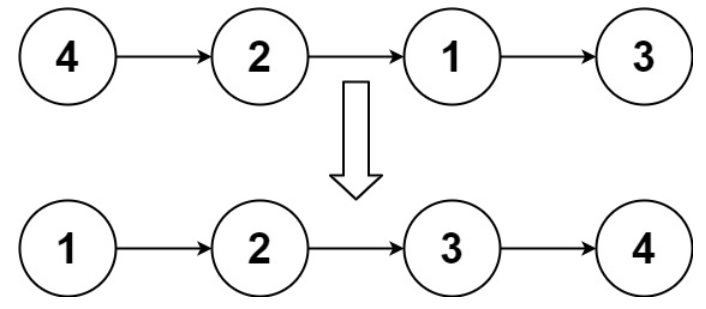
\includegraphics[width=0.5\linewidth]{figure/P6.png}
    \caption{For example}
    \label{fig:enter-label}
\end{figure}

\par For example, the street numbers of the old town are currently arranged as $[4, 2, 1, 3]$, with the head node $\textit{head} = 4$. You need to sort them in ascending order as $[1, 2, 3, 4]$.

\solution{
}
\newpage